\documentclass[a4paper, 10pt]{article}
\usepackage[utf8x]{inputenc}
\usepackage{graphicx}
\usepackage{geometry}
\usepackage{amsmath}
\usepackage{mathenv}
\usepackage{amssymb}
\usepackage{amsfonts}
\usepackage{mathrsfs}
\usepackage{textcomp}
\geometry{hmargin = 2.5cm, vmargin = 1.5cm}

% OPENING
\title{SY09 - TP04\\Analyses discriminantes quadratique et linéaire}
\author{Bertrand Bon - Antoine Hars}

\begin{document}

\maketitle

\section*{Introduction}
Dans le cadre de ce tp, nous avons étudié les analyses discriminantes quadratique et linéaire.\\ \\

\section*{Exercice 1 : Règle de Bayes.}
On suppose que la population est répartie en deux classes, en proportions $\pi_{1}$ et $\pi_{2}$ = 1 - $\pi_{1}$,
issues des distributions gaussiennes bivariées $\mathcal{N}(\mu_{1}, \Sigma_{1})$ et $\mathcal{N}(\mu_{1}, \Sigma_{1})$.\\

\subsection*{1. Donner une équation de la frontière de décision de la règle de Bayes dans chacun des cas suivants :}

\subsubsection*{(a) $\pi_{1}$ = 0.5, $\mu_{1}$ = (0,0)´, $\mu_{2}$ = (1,1)´, $\Sigma_{1}$ = $\Sigma_{2}$ =
$\begin{pmatrix} 1 & 0 \\ 0 & 1 \end{pmatrix}$ :}
% TODO

\subsubsection*{(b) $\pi_{1}$ = 0.1, $\mu_{1}$ = (0,0)´, $\mu_{2}$ = (1,1)´, $\Sigma_{1}$ = $\Sigma_{2}$ =
$\begin{pmatrix} 1 & 0 \\ 0 & 1 \end{pmatrix}$ :}
% TODO

\subsubsection*{(c) $\pi_{1}$ = 0.5, $\mu_{1}$ = (0,0)´, $\mu_{2}$ = (1,1)´, $\Sigma_{1}$ = $\Sigma_{2}$ =
$\begin{pmatrix} 1 & -0.3 \\ -0.3 & 1 \end{pmatrix}$ :}
% TODO

\subsubsection*{(d) $\pi_{1}$ = 0.6, $\mu_{1}$ = $\mu_{2}$ = (1,1)´, $\Sigma_{1}$ = $\begin{pmatrix} 1 & 0 \\ 0 & 1 \end{pmatrix}$,
$\Sigma_{2}$ =  $\begin{pmatrix} 5 & 0 \\ 0 & 5 \end{pmatrix}$ :}
% TODO

\subsubsection*{(e) $\pi_{1}$ = 0.6, $\mu_{1}$ = (0,0)´, $\mu_{2}$ = (1,1)´, $\Sigma_{1}$ = $\begin{pmatrix} 1 & 0 \\ 0 & 1 \end{pmatrix}$,
$\Sigma_{2}$ = $\begin{pmatrix} 1 & 0.5 \\ 0.5 & 1 \end{pmatrix}$ :}
% TODO

$\\ \\$
\subsection*{2. Simulation de la règle de Bayes dans R :}
Pour chacune des cinq populations précédentes, en utilisant la fonction \textit{simul} réalisée au TD3 (Théorie de la décision),
nous avons généré un échantillon de taille \textit{n} = 1000.\\
Pour rappel, le code de la fonction \textit{simul} est comme suit :\\
\begin{verbatim}
simul <- function (n, pi, mu1, mu2, sigma1, sigma2) {

  # On crée la matrice contenant l'échantillon résultat de la fonction.
  result = matrix(nrow = n, ncol = 3)

  # Affectation de chaque élément de l'échantillon final à la classe 0 ou 1.
  for (k in 1:n) {

    rand = sample(0:1, 1)
    result[k, 3] = rand

    if (result[k, 3] == 0) {
      result[k, c(1, 2)] = mvrnorm(1, mu1, sigma1)
    } else {
      result[k, c(1, 2)] = mvrnorm(1, mu2, sigma2)
    }
  }

  return (result)
}
\end{verbatim}
$\\ \\$
Pour chacun des échantillons de population, nous avons tracé les nuages suivants associés,
avec le tracé de la frontière de décision pour les trois premiers cas :\\
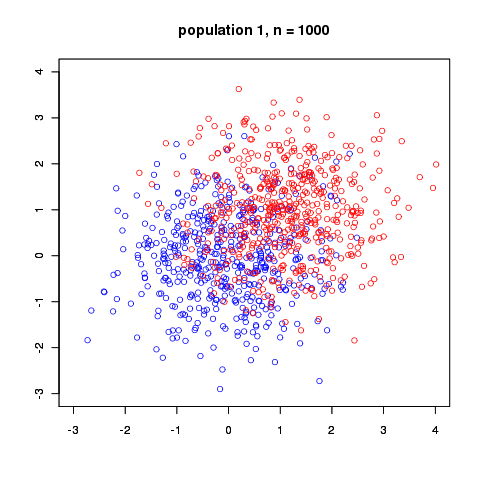
\includegraphics[height = 7cm, width = 7cm]{plots/exo1_simul_1.png}
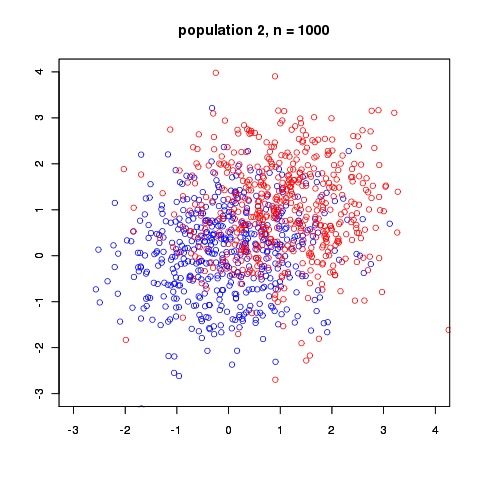
\includegraphics[height = 7cm, width = 7cm]{plots/exo1_simul_2.png}\\
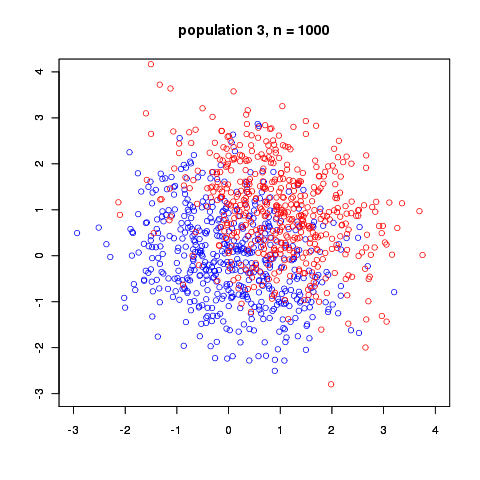
\includegraphics[height = 7cm, width = 7cm]{plots/exo1_simul_3.png}
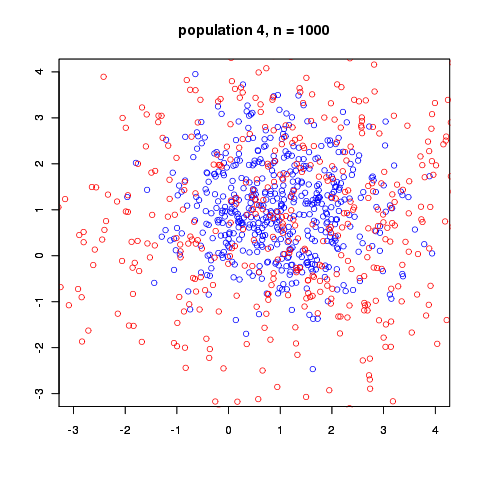
\includegraphics[height = 7cm, width = 7cm]{plots/exo1_simul_4.png}\\
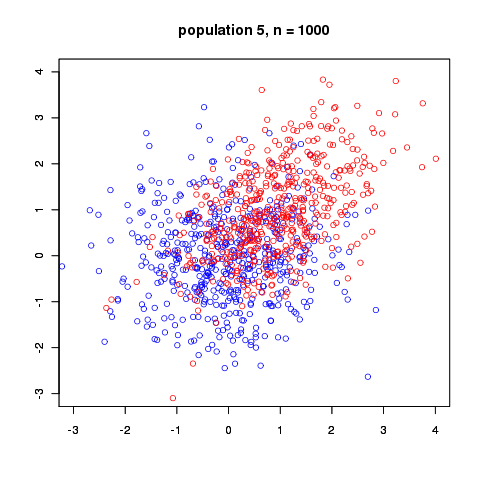
\includegraphics[height = 7cm, width = 7cm]{plots/exo1_simul_5.png}\\ \\
%TODO frontière de décision pour les 3 premiers cas.
Pour chaque cas de figure, nous avons déterminé l'expression d'un estimateur de la probabilité d'erreur,
ainsi que sa réalisation sur l'échantillon correspondant :\\
% TODO expression d'un estimateur de la probabilité d'erreur
Sa réalisation sur les échantillons nous donne les valeur suivantes :\\ \\
\begin{tabular}{|c|c|c|c|}
\hline
population & $\mu_{1}$ & $\mu_{2}$ & Probabilité d'erreur ($\%$) \\
\hline
1 & (-0.028, -0.093) & (1.062, 0.981) & 27.6 \\
\hline
2 & (0.346, 0.006) & (1.015, 0.982) & 31.1 \\
\hline
3 & (-0.063, -0.045) & (1.036, 0.915) & 30.6 \\
\hline
4 & (1.018, 0.919) & (1.221, 0.965) & 49 \\
\hline
5 & (-0.127, -0.018) & (1.001, 1.002) & 28.2 \\
\hline
\end{tabular}
$\\ \\$
Cela nous a permis de le comparer avec la probabilité d'erreur théorique.
% TODO probabilité d'erreur théorique

$\\ \\$
\section*{Exercice 2 : Analyse discriminante sur les données \textit{Crabes}.}
Dans cet exercice, nous désirons utiliser l'analyse discriminante linéaire et l'analyse discriminante quadratique sur les données \textbf{crabs}
afin de déterminer une fonction permettant de distinguer le sexe à partir des mesures \textit{FL} et \textit{RW}.\\

\subsection*{1. Expliquer ce que font les fonctions suivantes :}
\textbf{lda :} La fonction lda sert à effectuer l'analyse discriminante linéaire de données
(elle prend en paramètre une formule, un data frame ou une matrice).\\
Elle cherche à détecter si la matrice de covariance d'une classe est singulière.\\ \\
\textbf{qda :} Cette fonction est utilisée pour exécuter une analyse discriminante quadratique sur des données
en utilisant une décomposition QR qui retournera un message d'erreur si la variance du groupe est singulière pour chaque groupe.\\ \\
\textbf{contour :} Il s'agit d'une fonction générique utile pour créer un graphe de contour ou
pour ajouter des lignes de contour à un graphe existant.\\ \\
\textbf{sample :} Cette fonction nous permet de récupérer un échantillon de taille spécifiée d'éléments de l'ensemble X
en remettant en place ou non les éléments.\\ \\
\textbf{predict :} Predict() est une fonction générique de prédictions à partir des résultats des diverses fonctions de création de modèles.
La forme retournée dépend de la classe entrée en paramètre.\\ \\
\textbf{predict.lda :} Cette fonction classifie des observations multi-variables en utilisant l'analyse discrimante linéraire et
projette les données sur les discriminantes linéaires.
Cette fonction centre les discriminants linéaires de sorte que le nombre moyen pondéré des centres de gravité du groupe soit à l'origine.\\ \\
\textbf{Comparaison entre predict et predict.lda :} predict.lda est une méthode de la fonction générique predict pour la class lda.
On peut soit appeler predict() sur une classe lda d'un objet spécifié ou
appeler la fonction predict.lda() sans se soucier de la classe de l'objet.\\ \\

\subsection*{2.}

\subsection*{3.}

\subsection*{4. }

\section*{Exercice 3 : }

\subsection*{}
\subsection*{}
\subsection*{}

\section*{Conclusion}

\end{document}
